\documentclass[11pt,letterpaper]{article}

\usepackage[T1]{fontenc}
\usepackage{mathpazo}
\usepackage{microtype}
\usepackage[margin=1in]{geometry}
\usepackage{titlesec}
\usepackage{fancyhdr}
\usepackage{booktabs}
\usepackage{tabularx}
\usepackage{epigraph}
\usepackage{hyperref}

\usepackage{tikz}
\usetikzlibrary{arrows.meta, positioning, calc, shapes.geometric, backgrounds, fit}

% Define colors
\definecolor{accent}{HTML}{2E4057}
\definecolor{midgray}{HTML}{6B7280}
\definecolor{teal}{HTML}{0D7377}
\definecolor{deepred}{HTML}{9B2335}
\definecolor{deepblue}{HTML}{1E3A5F}

% Hyperref setup
\hypersetup{
  colorlinks=true,
  linkcolor=accent,
  citecolor=accent,
  urlcolor=teal
}

% Header and footer
\pagestyle{fancy}
\fancyhf{}
\rhead{\textcolor{midgray}{\thepage}}
\lhead{\textcolor{midgray}{The Meta-Method}}
\cfoot{}
\renewcommand{\headrulewidth}{0.5pt}
\renewcommand{\headrule}{\color{midgray}\hrule}

% Section formatting
\titleformat{\section}
  {\Large\bfseries\color{deepblue}}
  {\thesection.}
  {0.5em}
  {}
  [\vspace{0.3em}\textcolor{teal}{\titlerule[2pt]}]

\titleformat{\subsection}
  {\large\bfseries\color{accent}}
  {\thesubsection.}
  {0.5em}
  {}

\titlespacing{\section}{0pt}{1.5em}{0.8em}
\titlespacing{\subsection}{0pt}{1em}{0.6em}

% Epigraph formatting
\setlength{\epigraphwidth}{0.7\textwidth}

\title{\Huge\textcolor{deepblue}{The Meta-Method}\\\vspace{0.5em}\large\textcolor{accent}{Theseus as a Theory of Inquiry}}
\author{\textcolor{midgray}{Theseus Intellectual Capital}}
\date{\textcolor{midgray}{April 2026}}

\begin{document}

\maketitle

\begin{center}
\textit{\textcolor{midgray}{Internal Working Document}}
\end{center}

\vspace{2em}

% ============================================================================
% READER'S GUIDE
% ============================================================================

\section*{A Reader's Guide}

\noindent Most people and organizations ask a single, urgent question: \textbf{What is true?}

They want answers. Facts. Conclusions they can act on. This is natural. It is also, we believe, a trap.

Theseus asks a different question: \textbf{How can we reliably figure out what is true?}

This is not a retreat from the first question — it is a more sophisticated version of it. Because the truth is that anyone can make a claim. The interesting problem is distinguishing between a claim that happens to be right (because of luck or accident) and a claim that was \emph{arrived at through a reliable process}. The second kind of claim is worth building on. The first kind is not.

This document explains why that distinction matters, what a reliable truth-finding method looks like, and how you can evaluate whether your own reasoning — or your organization's reasoning — is actually working.

We begin with three orders of abstraction: from substantive claims about the world, to the methods we use to discover truth, to a theory of what makes methods reliable. Most of the document is devoted to five formal criteria that any reliable method should satisfy. We then show how these criteria map onto a firm's actual work, and address the deepest question: can a method evaluate itself?

\textbf{For the philosopher:} This document draws on Lakatos, Laudan, Mayo, Solomonoff, Popper, and the No Free Lunch theorems. It is a synthesis, not an original contribution to philosophy of science. What makes it distinctive is that it has been made computational and applied to a firm's reasoning.

\textbf{For the practitioner:} This document is not abstract. Each criterion has a concrete diagnostic. We show how to measure progressivity, severity, coherence, compressibility, and domain sensitivity in your own work. Every claim in this document can be tested.

\textbf{For the skeptic:} Read the objections section. We engage seriously with the strongest criticisms. Yes, this is philosophy of science repackaged. Yes, it is abstract. Yes, some of it may seem useless. We address all three objections and explain why we believe we are wrong about those things.

---

\newpage

\tableofcontents

\newpage

% ============================================================================
% 1. THE THREE ORDERS
% ============================================================================

\section{The Three Orders of Abstraction}

The firm has moved through three levels of abstraction. Each is a genuine advance, and it is worth being precise about why.

\subsection*{First Order: Substantive Claims}

\noindent \textbf{``We believe X is true.''}

This is where most firms, thinkers, and investors operate. The product is a claim about the world. The product has immediate appeal — it is actionable. You can bet on it. You can build a strategy around it.

The vulnerability is obvious: if X turns out to be false, the entire edifice collapses. A fund that bets on a specific thesis is only as good as that thesis. An organization whose reputation rests on a substantive claim is one crisis away from collapse.

Worse: the organization has no way to learn from failure. If the claim was wrong, was it because the claim itself was false, or because the reasoning process that led to the claim was flawed? These are fundamentally different diagnoses, and they require fundamentally different responses. But at the first order, you cannot distinguish between them.

\subsection*{Second Order: Methodology}

\noindent \textbf{``We have a reliable method for determining whether X is true.''}

This is stronger. The product is not a specific claim but a procedure — a process, an algorithm, a coherence engine, a contradiction detector. If X turns out to be false, and the method is sound, the method should catch it. The method becomes a second order of defense.

The vulnerability here is more subtle: the method itself might be unreliable. A coherence engine that mismeasures coherence is worse than useless; it is confidently wrong. An organization can follow its own methodology faithfully and still systematically arrive at false conclusions.

At the second order, you have a way to learn from failure: you can diagnose whether the failure was in the method itself or in the application of the method. But you still cannot be sure.

\subsection*{Third Order: Meta-Methodology}

\noindent \textbf{``We have a theory of what makes a method reliable, and we can evaluate competing methods by this theory.''}

This is what Theseus is now reaching for. The product is not a claim or a method but a \emph{criterion for evaluating methods}. The question is no longer ``which path through the maze?'' or ``which pathfinding algorithm?'' but ``what formal properties must any pathfinding algorithm possess in order to be reliable, and how do we determine this for any given class of problems?''

This third order is where the deepest intellectual action is. It is also the most abstract. But abstraction, at this level, is the only way to escape the cycle of confident error.

---

\newpage

% ============================================================================
% 2. THE MAZE ANALOGY, EXTENDED
% ============================================================================

\section{The Maze Analogy: Four Levels of Navigation}

Consider four agents trying to navigate a maze. Each operates at a different level of abstraction. This analogy illuminates the structure of inquiry itself.

\subsection*{The Dogmatist}

The dogmatist \textbf{knows the path}. ``Turn left at the first fork, then right at the second, then straight ahead.'' The dogmatist has memorized the solution. This works perfectly — until the maze changes.

In inquiry, the dogmatist is the person who has been told what to believe (by tradition, authority, or intuition) and defends that belief against all evidence. The dogmatist's reasoning is not adaptive. It cannot learn. It is brittle.

\subsection*{The Methodologist}

The methodologist \textbf{has an algorithm}. ``At each fork, face the exit's approximate direction and move toward it. If you hit a dead end, backtrack and try the next branch.'' This is a rule of thumb, a heuristic. It works for many mazes — mazes where the exit is vaguely visible, mazes that do not have long detours that point toward the false exit.

But the methodologist's algorithm fails for mazes where the direct path leads to dead ends. It fails for mazes where the optimal path requires taking a detour that \emph{moves you farther} from the exit before bringing you closer. The methodologist knows a single algorithm and tries to apply it everywhere.

In inquiry, the methodologist is the person who has learned a procedure (statistical hypothesis testing, peer review, logical deduction) and applies it faithfully. This is better than being a dogmatist — the algorithm can adapt to new mazes. But the algorithm is not infinitely flexible.

\subsection*{The Meta-Methodologist}

The meta-methodologist \textbf{evaluates algorithms}. ``A* search with admissible heuristics is provably optimal for shortest-path problems in fully observable environments. But in partially observable environments, POMDP-based planning outperforms A*. In adversarial environments, minimax search is more robust. The choice of algorithm depends on the structure of the problem.'' This agent does not commit to one algorithm; it knows which algorithm to deploy under which conditions.

The meta-methodologist recognizes the NFL theorem (discussed below): no algorithm is universally optimal. But the NFL theorem does not say all algorithms are equally good for a given problem. It says that across all possible problems, they average out. On a specific problem class, one algorithm dominates.

In inquiry, the meta-methodologist is the person who knows that case studies work better for understanding complexity, that randomized trials work better for isolating causal mechanisms, that historical analysis works better for understanding change over time. This agent can recognize the structure of the problem at hand and select the method accordingly.

\subsection*{The Theorist of Inquiry}

The theorist of inquiry asks: \textbf{``What formal properties must ANY reliable pathfinding algorithm have, regardless of the maze? And what determines which properties are necessary for which classes of mazes?''}

This agent does not select an algorithm. Instead, it builds a map of domains and algorithms. It asks: what must we know about a maze before we can say which algorithm will work best? What properties of the algorithm itself guarantee reliability in its designated domain?

In inquiry, the theorist of inquiry is asking: ``Across all the methods that work — across case studies and trials and simulations and historical analysis — what do they have in common? What formal properties do reliable methods possess?'' This is the level at which Theseus operates.

\subsection*{Visualizing the Four Levels}

\vspace{1em}

\begin{center}
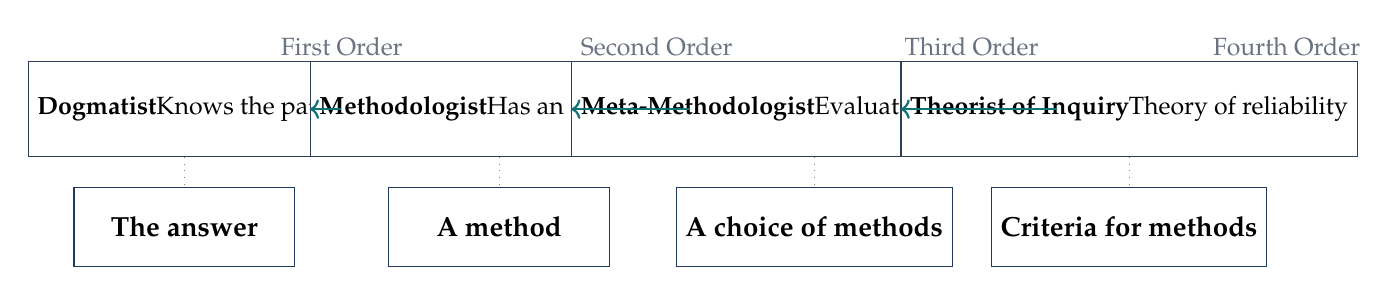
\begin{tikzpicture}[
  level/.style={draw=none},
  box/.style={rectangle, draw=accent, fill=white, minimum width=3cm, minimum height=1.2cm, text centered, font=\small},
  level box/.style={rectangle, draw=deepblue, fill=white, minimum width=2.8cm, minimum height=1cm, text centered, font=\footnotesize, font=\bfseries},
]

  % Dogmatist
  \node[box] (d) at (0, 0) {\textbf{Dogmatist}\\Knows the path};
  \node[level box] (d2) at (0, -1.5) {The answer};

  % Methodologist
  \node[box] (m) at (4, 0) {\textbf{Methodologist}\\Has an algorithm};
  \node[level box] (m2) at (4, -1.5) {A method};

  % Meta-Methodologist
  \node[box] (mm) at (8, 0) {\textbf{Meta-Methodologist}\\Evaluates algorithms};
  \node[level box] (mm2) at (8, -1.5) {A choice of methods};

  % Theorist
  \node[box] (t) at (12, 0) {\textbf{Theorist of Inquiry}\\Theory of reliability};
  \node[level box] (t2) at (12, -1.5) {Criteria for methods};

  % Arrows
  \draw[->, thick, teal] (d) -- (m);
  \draw[->, thick, teal] (m) -- (mm);
  \draw[->, thick, teal] (mm) -- (t);

  % Vertical lines
  \draw[dotted, gray] (d) -- (d2);
  \draw[dotted, gray] (m) -- (m2);
  \draw[dotted, gray] (mm) -- (mm2);
  \draw[dotted, gray] (t) -- (t2);

  % Labels
  \node[font=\small, color=midgray] at (2, 0.8) {First Order};
  \node[font=\small, color=midgray] at (6, 0.8) {Second Order};
  \node[font=\small, color=midgray] at (10, 0.8) {Third Order};
  \node[font=\small, color=midgray] at (14, 0.8) {Fourth Order};

\end{tikzpicture}
\end{center}

\vspace{1em}

The progression shows increasing abstraction, but also increasing robustness. The dogmatist is brittle; one false belief breaks everything. The theorist of inquiry is adaptive; it can evaluate new methods as they emerge.

---

\newpage

% ============================================================================
% 3. FIVE CRITERIA
% ============================================================================

\section{Five Criteria for Evaluating Methods}

Drawing on the research traditions of Lakatos, Laudan, Mayo, Solomonoff, and the No Free Lunch theorems, we now present five formal properties that any reliable truth-finding method should possess. These are the criteria by which Theseus evaluates any methodology — its own or anyone else's.

% ============================================================================
% 3.1 PROGRESSIVITY
% ============================================================================

\subsection{Criterion 1: Progressivity (Lakatos)}

\subsubsection*{The Core Idea}

A method is \textbf{progressive} if it generates novel, testable predictions that go beyond what initially motivated the method. A method is \textbf{degenerating} if it only produces post-hoc explanations of what is already known.

Imre Lakatos developed this distinction to solve a puzzle in the history of science. Newton's theory of gravitation made stunning new predictions: it predicted the existence of Neptune before that planet was ever observed. By contrast, Marxist theory, in Lakatos's view, seemed to explain everything \emph{after the fact}. Every historical event could be fitted into the Marxist framework, but the theory appeared to make no novel predictions about the future. One seemed like good science; the other seemed like dogmatism dressed in scientific language.

Progressivity is the distinction between these two.

\subsubsection*{What Lakatos Actually Said}

Lakatos described science not as a collection of isolated theories but as \emph{research programmes}. A research programme consists of:

\begin{itemize}
  \item A \textbf{hard core} — the fundamental, untouchable assumptions that define the programme. For Newton, this was the law of gravitation and the axioms of motion.
  \item A \textbf{protective belt} of auxiliary hypotheses that can be modified when the hard core is threatened. When observations conflict with the theory, the methodologist adds auxiliary hypotheses to preserve the core.
  \item A \textbf{positive heuristic} — a sense of what directions are fruitful to pursue, what problems are worth solving.
\end{itemize}

A research programme is \textbf{progressive} if:
\begin{enumerate}
  \item It generates new, unexpected predictions.
  \item These predictions are eventually confirmed (at least some of them).
  \item The auxiliary hypotheses needed to explain the new observations are not \emph{ad hoc} — they seem natural extensions of the core.
\end{enumerate}

A research programme is \textbf{degenerating} if:
\begin{enumerate}
  \item It explains past observations but fails to predict new ones.
  \item When it does make predictions, they fail.
  \item It responds by adding increasingly \emph{ad hoc} auxiliary hypotheses — special-case explanations that only work for the cases that failed.
\end{enumerate}

The intuition is this: a true theory will reveal deeper structure and generate new predictions. A false theory will require constant patching.

\subsubsection*{Historical Examples}

\textbf{Newton's Gravitational Programme (Progressive):}

Newton's theory began with a simple core: $F = ma$ and $F = Gm_1m_2/r^2$. From this, astronomers derived the orbits of known planets. But the theory also made a striking prediction: if the sun's gravity can bend light (a later refinement), then light from stars should be bent as it passes near the sun. This prediction was confirmed during the solar eclipse of 1919, and it won converts to Einstein's version of gravitational theory.

The key point: Newton's theory did not merely explain the planets that were already known. It generated a novel prediction about a phenomenon (Neptune's existence) that was subsequently observed. This is progressivity.

\textbf{Marxist Historical Theory (Degenerating, in Lakatos's view):}

Lakatos claimed that Marxist theory explained every historical event — feudalism gave way to capitalism because of the laws of historical materialism; capitalism will give way to communism for the same reason. But when predictions failed (the revolution did not occur in industrialized countries; the working class did not become poorer), the theory simply added new epicycles: the revolution was delayed because of imperialism, or trade unionism, or the national bourgeoisie. The hard core was never questioned; new auxiliary hypotheses were always invented.

The key point: Marxist theory excelled at explanation after the fact but failed at prediction. This is degeneracy.

\textbf{Freudian Psychoanalysis:}

Freud's theory of the unconscious mind was initially progressive. It explained dreams, slips of the tongue, and symptoms of neurosis. But as it developed, every possible human behavior became evidence for the theory. Did someone deny having a repressed desire? This was explained as repression itself. The theory became unfalsifiable.

\subsubsection*{The Progressivity Test for a Firm}

Apply this to your own work:

\begin{enumerate}
  \item \textbf{Identify your method's hard core.} What are the fundamental assumptions? (``All value comes from competitive advantage.'' ``Technology adoption follows S-curves.'')
  \item \textbf{List your method's predictions.} What would the method predict about situations you have not yet observed?
  \item \textbf{Check: are these predictions novel?} Do they go beyond what already motivated the method? Or are you just deriving things that were implicit in the initial motivation?
  \item \textbf{Check: do the predictions come true?} When you make a forecast using the method, how often is it correct? (This is progressivity's empirical test.)
  \item \textbf{Check: when predictions fail, do you patch the core or the protective belt?} If failures require changing the fundamental assumptions, this is a sign of degeneracy. If failures can be absorbed by modifying auxiliary hypotheses in natural ways, this is a sign of progressivity.
\end{enumerate}

Many organizations fail this test. They have a thesis, and every event is explained as confirming the thesis. Tech is disrupting everything, so even setbacks in tech are explained as signs of disruption. Or: the markets are overvalued, so bull markets are explained as temporary aberrations. The method explains everything, predicts nothing, and is therefore degenerate.

\subsubsection*{Objections and Refinements}

One objection: the notion of a ``novel'' prediction is ambiguous. Is a prediction novel if it is novel in time (not made before the observation) or novel in logic (not deducible from the prior theory)? Lakatos himself struggled with this. A clever enough logician can always show that a ``new'' prediction was implicit in the old theory.

Another objection: a programme can resurrect. A programme that was degenerating for decades can suddenly become progressive again if new tools or evidence emerge. Lakatos allows for this; his criterion is not about a programme's eternal status but about its trajectory.

The key insight remains: distinguish between a method that is generating novel insights and a method that is generating novel excuses.

\subsubsection*{Connection to the Other Criteria}

Progressivity is necessary but not sufficient. A method can be progressive and yet produce beliefs that are not actually true — it just happens to predict things, and those predictions happen to come true by accident. This is why we need the other four criteria. Severity asks: would the method have detected falsity? Coherence asks: do the method's assumptions align with its aims? Compressibility asks: is the method parsimonious? Domain sensitivity asks: are we applying the method in its proper domain?

---

\newpage

\subsection{Criterion 2: Severity (Mayo)}

\subsubsection*{The Core Idea}

\textbf{Severity}, as developed by Deborah Mayo, is about how hard a test is. Evidence supports a claim only if the test had a high probability of revealing the claim's falsity, had the claim been false.

This is counterintuitive, so let's start with an analogy.

\subsubsection*{The Bridge Analogy}

Imagine you build a bridge and want to test whether it can hold 10 tons. You place a 1-pound feather on the bridge, and it does not collapse. Does this test \emph{severely} support the claim that the bridge holds 10 tons?

No. A 1-pound test would pass almost any bridge, including a very weak bridge. So the test does not tell you much about whether the bridge can actually hold 10 tons.

Now imagine you place a 9-ton load on the bridge, and it holds. This is a much severer test. It would probably have failed if the bridge could only hold 5 tons. So a successful result in this test provides strong evidence that the bridge can hold at least 9 tons.

Severity is about using the hardest test that can feasibly be applied. A test is severe if it would probably have caught you in an error, had you been making one.

\subsubsection*{Formal Definition}

Let $C$ be a claim (e.g., ``the bridge holds 10 tons''), let $E$ be evidence (e.g., ``the bridge held a 9-ton load''), and let $D$ be a test or experiment.

A test $D$ severely supports $C$ given $E$ if:
\begin{enumerate}
  \item The evidence $E$ is consistent with $C$.
  \item The probability that the test $D$ would have produced evidence that \emph{falsifies} $C$, if $C$ were false, is high.
\end{enumerate}

In short: the method would have caught the error if the error existed.

\subsubsection*{Historical Examples}

\textbf{Clinical Trials:}

A randomized controlled trial with a large sample size is a severe test. If a drug does not actually work, the trial would (with high probability) detect this. So if the trial shows the drug works, we have strong evidence for the claim.

By contrast, a trial with a tiny sample size is non-severe. Even if the drug does not work, a small sample might (by chance) show positive results. So positive results in a small trial are weak evidence.

\textbf{Observational Studies:}

Suppose we observe that people who exercise live longer than people who do not exercise. Does this severely support the claim that exercise causes longevity?

No. This test would pass even if exercise does not cause longevity — perhaps healthier people are more likely to exercise, and their health (not the exercise) causes them to live longer. The test does not distinguish between the two hypotheses. Therefore, it is non-severe for the causal claim.

A severe test would have to rule out the alternative. For instance, a randomized trial (assigning people to exercise or no-exercise groups) would be more severe, because it would tend to produce different results if exercise did not cause longevity.

\textbf{The Replication Crisis in Psychology:}

Many published psychological studies are non-severe. A psychologist tests a hypothesis on a small sample, finds a $p$-value less than $0.05$, and publishes. But a $p < 0.05$ test is barely severe — it means only that the observed result would occur less than 5\% of the time if the hypothesis were false. With small sample sizes, noise can easily produce a false positive.

When other researchers tried to replicate these studies, many failed. This revealed that the original tests were not severe: they did not have a high enough probability of detecting falsity, because the sample sizes were too small.

\subsubsection*{The Severity Test for a Firm}

Apply this to your own analysis:

\begin{enumerate}
  \item \textbf{State the claim clearly.} (``Company X has a durable competitive moat.'')
  \item \textbf{Describe the test.} What analysis did you perform? What data did you examine?
  \item \textbf{Ask: would this test have caught the opposite conclusion?} If the claim were false — if company X did \emph{not} have a durable moat — would your test have revealed this? Or would the test pass under almost any condition?
  \item \textbf{Look for easy outs.} Can you explain the evidence in multiple ways? If so, the test is non-severe. A severe test rules out alternative explanations.
  \item \textbf{Increase the difficulty.} Can you apply a more rigorous test? Can you explicitly try to falsify the claim? Can you generate predictions the claim makes and check them?
\end{enumerate}

Most analysis fails this test. A research report compiles evidence that supports a conclusion, and the analyst believes the conclusion is proven. But the analysis never examines what would disconfirm the conclusion. A severe analysis would say: ``Here is what would have to be true for my conclusion to be false. And here is why those things are not true.''

\subsubsection*{Connection to Progressivity}

Progressivity and severity are complementary. A progressive method generates novel predictions. Severity asks whether those predictions can actually test the method or whether they are guaranteed to come out true regardless.

Ideally, a method is both progressive (generates novel predictions) and severe (those predictions would distinguish the method from competitors). A method that generates boring predictions is not progressive. A method that generates predictions that would pass anyway is not severe.

---

\newpage

\subsection{Criterion 3: Coherence (Laudan)}

\subsubsection*{The Core Idea}

\textbf{Coherence}, in Larry Laudan's framework, is different from simple logical consistency. A set of claims is consistent if they do not contradict each other. But they can be consistent without being coherent.

Coherence is about fit across different levels: between aims (what you are trying to accomplish), methods (how you are trying to accomplish it), and theories (your beliefs about the world). These three must support each other.

\subsubsection*{Laudan's Reticulated Model}

Laudan's central insight is that aims, methods, and theories are \textbf{mutually supporting}. They form a triangle:

\begin{center}
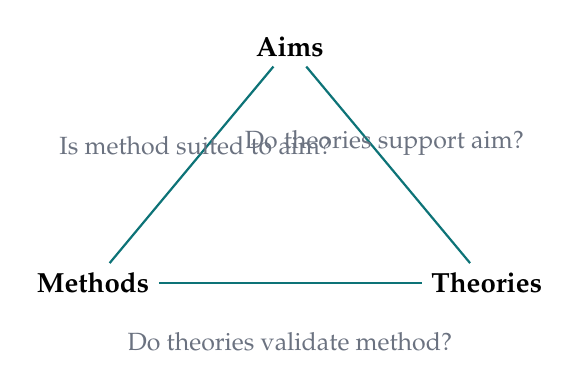
\begin{tikzpicture}[
  triangle/.style={draw=deepblue, thick, minimum size=3cm},
]

  \node (a) at (0, 3) {\textbf{Aims}};
  \node (m) at (-2.5, 0) {\textbf{Methods}};
  \node (t) at (2.5, 0) {\textbf{Theories}};

  \draw[thick, teal, -] (a) -- (m);
  \draw[thick, teal, -] (a) -- (t);
  \draw[thick, teal, -] (m) -- (t);

  \node[font=\small, color=midgray, anchor=south] at (-1.2, 1.5) {Is method suited to aim?};
  \node[font=\small, color=midgray, anchor=south] at (1.2, 1.5) {Do theories support aim?};
  \node[font=\small, color=midgray, anchor=north] at (0, -0.5) {Do theories validate method?};

\end{tikzpicture}
\end{center}

For example:

\textbf{Aristotelian Science (Medieval Period):}
\begin{itemize}
  \item \textbf{Aim:} Achieve certainty about the essences of things.
  \item \textbf{Method:} Logical deduction from self-evident first principles.
  \item \textbf{Theory:} Everything has an essential nature; logic can reveal these natures.
\end{itemize}

These three cohere. The method (logical deduction) is well-suited to the aim (certainty), and the theory (essentialism) supports both the aim and the method.

\textbf{Galilean Science (Scientific Revolution):}
\begin{itemize}
  \item \textbf{Aim:} Develop predictive models of the natural world (not certainty, but accuracy).
  \item \textbf{Method:} Experimentation combined with mathematical modeling.
  \item \textbf{Theory:} The world operates according to mathematical laws; not all properties need to be essential.
\end{itemize}

Again, these cohere. The method (experimentation) is well-suited to the aim (prediction), and the theory (mathematical laws) supports both.

\subsubsection*{Coherence Failures}

A coherence failure occurs when these three pull in different directions.

\textbf{Example 1:} A firm's stated aim is ``identify companies with durable competitive advantages.'' Its method is ``compare P/E ratios to sector averages.'' There is a coherence failure: the method does not address the aim. P/E ratios are valuation metrics; they do not tell you whether an advantage is durable. A method suited to the aim would involve analyzing the sources of the advantage (network effects, switching costs, scale economies, etc.) and forecasting whether those sources persist.

\textbf{Example 2:} A research organization's aim is ``understand the mechanisms of climate change.'' Its method is ``conduct large-scale statistical studies of weather patterns.'' Its theory is ``climate is determined entirely by random chaos, and therefore no mechanism exists.'' The theory contradicts the aim: if you believe there is no mechanism, you will not find one. The method is non-severe for the aim: it can reveal correlations but not mechanisms.

\subsubsection*{The Pessimistic Meta-Induction}

Laudan addressed a famous objection: most past scientific theories have turned out to be false. So probably ours are too. This is the ``pessimistic meta-induction.''

His response: we should be pessimistic about theories, but not about methods. Newton's theory of gravity was (in some sense) false — Einstein showed it was a special case of a more general theory. But Newton's method of combining observation with mathematics was not false; it was an advance.

This insight is crucial for understanding Theseus. The firm will sometimes be wrong about specific claims. But the meta-method — the process by which we evaluate methods — should improve over time, even as specific theories change.

\subsubsection*{The Coherence Test for a Firm}

\begin{enumerate}
  \item \textbf{State your aims clearly.} What are you trying to accomplish? (Maximize returns? Discover truth? Help others?)
  \item \textbf{Describe your methods.} What procedures do you use?
  \item \textbf{List your theories.} What beliefs about the world do you hold?
  \item \textbf{Check aim-method fit:} Does the method actually accomplish the aim? Or are you using a method that would be appropriate for a different aim?
  \item \textbf{Check aim-theory fit:} Do your beliefs support your aims? If you believe X, does that make your aim more or less likely to be achieved?
  \item \textbf{Check method-theory fit:} Do your theories justify your method? Does your method rest on assumptions that your theories contradict?
  \item \textbf{If you find a failure, decide what to change:} You can change your aim (redefine what you are trying to do), change your method (adopt a different procedure), or change your theory (revise your beliefs). But you must restore coherence.
\end{enumerate}

\subsubsection*{When Aims Conflict}

A sophisticated version of the coherence test asks: what if you have multiple, conflicting aims?

For example: a firm might aim to both (1) discover truth and (2) make money. These aims sometimes conflict. When they do, the firm must be explicit about the trade-off. It cannot claim to be pursuing both aims equally while using a method that optimizes for only one.

This is a case where coherence requires honesty.

---

\newpage

\subsection{Criterion 4: Compressibility (Solomonoff and Kolmogorov)}

\subsubsection*{The Core Idea}

The best explanation is the shortest one that accounts for all the data. This is Occam's Razor, but made precise.

\textbf{Kolmogorov complexity} is the length of the shortest computer program that produces a string of data. The \textbf{Kolmogorov complexity} of a dataset is a measure of how incompressible it is — how much information you need to describe it.

A good explanation is a short program that generates all the data. A bad explanation requires many special cases, many parameters, many exceptions.

\subsubsection*{Solomonoff Induction}

Ray Solomonoff imagined an ideal Bayesian reasoner — a mathematical idealization. This reasoner receives a sequence of observations and updates its beliefs about the underlying rule that generated the sequence.

Solomonoff showed that the ideal reasoner would assign higher probability to shorter programs. This is not an assumption; it is a consequence of Bayesian logic combined with the notion that shorter programs are more likely (in a specific technical sense).

The result is \textbf{Solomonoff induction}: a formal version of Occam's Razor. If two hypotheses explain the data equally well, the shorter one is (all else equal) more likely to be true.

\subsubsection*{Minimum Description Length}

In practice, Kolmogorov complexity is uncomputable. But we can approximate it using \textbf{Minimum Description Length (MDL)} — the length of a description using a specific language (e.g., English, or a specific data compression algorithm).

For example:

\textbf{Bad Explanation:} ``Company X succeeded because of factor A. Company Y succeeded because of factor B. Company Z succeeded because of factor C. Company W succeeded because of factor D. Company V succeeded because of factors A and E. Company U...'' This explanation requires a separate clause for each data point. It is not compressible. It is a list, not a theory.

\textbf{Good Explanation:} ``Companies succeed when they have a sustainable competitive advantage that competitors cannot easily replicate.'' This explanation is short and generates all the data (in principle). If the theory is true, we can explain each company's success as either having such an advantage or not having one.

The length is the difference: the bad explanation is as long as the data itself. The good explanation is much shorter.

\subsubsection*{Historical Examples}

\textbf{Newton vs. Ptolemy:}

Ptolemy's theory required a different epicycle (a small circle whose center moves on a larger circle) for each planet. Each epicycle had to be carefully calibrated to fit the observations. The theory fit the data, but it required many parameters, many special adjustments.

Newton's theory required three laws and one equation: $F = Gm_1m_2/r^2$. These few principles generated the motions of all the planets. This is compressibility.

Did Newton's theory come to be accepted because it was more compressible? Not only because of that — but compressibility was part of the argument. The theory was more elegant, required fewer assumptions, generated more predictions.

\textbf{Evolution vs. Special Creation:}

Before Darwin, biologists invoked special creation: God created each species separately, each perfectly adapted to its niche. This explained the data (the existence of adapted organisms) but required a separate creative act for each species.

Darwin's theory required one mechanism (natural selection) operating over time. This generated the diversity of life without requiring separate explanations for each species. It was more compressible.

The compressibility argument is not proof of truth — it is an epistemic bet that simpler theories are more likely to be right.

\subsubsection*{The Compressibility Test for a Firm}

\begin{enumerate}
  \item \textbf{State your thesis.} What is your core claim?
  \item \textbf{Count the number of premises.} How many assumptions does the thesis require?
  \item \textbf{Count the number of phenomena explained.} How many observations does the thesis account for?
  \item \textbf{Compute the ratio:} premises / explained phenomena. A ratio of 1:1 is bad (you have a list, not a theory). A ratio of 1:10 or better is good.
  \item \textbf{Look for special cases.} Does your thesis require many qualifications? (``In most cases X happens, except when Y. And in those cases, usually Z, except when....'') Each qualification reduces compressibility.
  \item \textbf{Simplify.} Can you restate the thesis more concisely? Can you remove assumptions that are not doing work?
\end{enumerate}

Many investment theses fail this test. The thesis might be: ``Tech companies will disrupt traditional industries.'' But the fund finds that different tech companies succeed in different ways, under different conditions, in different industries. So it adds: ``Disruption happens in industries where X, Y, and Z are true.'' Then: ``But also, in some cases where X is false, disruption still happens because of A.'' Etc. The thesis becomes a collection of special cases.

A compressible thesis would identify the core mechanism and state the conditions under which it applies.

\subsubsection*{Criticisms and Limitations}

One objection: Kolmogorov complexity is uncomputable. We cannot actually calculate it for a real hypothesis. Therefore, Solomonoff induction is beautiful in theory but useless in practice.

Response: True. But MDL is a practical approximation, and simpler theories really do tend to generalize better. There is empirical evidence for this.

Another objection: simplicity is not always truth. A simpler theory might miss important causal factors. Sometimes a more complex theory is actually more accurate.

Response: True. But the hypothesis-space is infinite. If we treat all hypotheses as equally likely, we can never learn anything. Some prior bias toward simplicity is necessary. Solomonoff's insight is that this bias has a formal justification.

---

\newpage

\subsection{Criterion 5: Domain Sensitivity (No Free Lunch)}

\subsubsection*{The Core Idea}

The \textbf{No Free Lunch (NFL) theorem} is one of the most important results in machine learning and the theory of learning. It says: no learning algorithm outperforms random guessing when averaged across all possible problem instances.

This sounds catastrophic. But its actual meaning is more subtle and more interesting.

\subsubsection*{What the NFL Theorem Actually Says}

Imagine a learning algorithm $A$ and a problem domain $D$. The algorithm $A$ does well on some problems in $D$ and poorly on others. If we average $A$'s performance across all possible problems (all possible strings of data), $A$ does no better than a random guesser.

Why? Because for every problem on which $A$ does well, there is a problem on which $A$ does poorly (roughly, the exact opposite problem). Averaged across all possibilities, these balance out.

But here is the key: this average is across \textbf{all possible} problem instances, weighted equally. In reality, we do not encounter all possible problems. We encounter specific problem domains.

Within a specific domain, algorithms can differ dramatically. For drug testing, randomized controlled trials are far superior to casual observation. For understanding complex historical events, case studies are superior to statistical models. The NFL theorem does not say algorithms are equal within a domain; it says they average to equal across \textbf{all} domains.

\subsubsection*{What This Means}

The NFL theorem implies a powerful conclusion: \textbf{every method has a domain}. There is no universal method. But domains matter.

The meta-methodologist's job is to map methods to domains. For each domain the firm encounters, identify which method is most reliable.

\subsubsection*{Examples}

\textbf{Randomized Controlled Trials:}

RCTs are excellent for isolating causal effects in well-defined settings. Do this drug reduce blood pressure? Does this teaching method improve test scores? These are questions where RCTs shine.

But RCTs are terrible for understanding why something works, in complex systems, or when the intervention is large-scale. You cannot randomize economic policies across countries to test their causal effects. RCTs fail in these domains.

\textbf{Case Studies:}

Case studies are excellent for understanding complex systems, generating hypotheses, and exploring mechanisms. How did Amazon become dominant? Why did the Soviet Union collapse? Case studies can generate rich explanations.

But case studies do not establish causation reliably (you can always tell an alternative story) and do not generalize well. A single case study of one company does not tell you much about other companies.

\textbf{Statistical Models:}

Statistical models are excellent for finding patterns in large datasets and making predictions in well-behaved domains (normal distributions, no tail risks). But they are terrible in domains with extreme events (fat tails, black swans). A statistical model trained on historical market returns will be blindsided by a market crash that is more extreme than historical precedent.

\subsubsection*{The Domain Boundary Problem}

The challenge is: how do you know when you have left your method's home turf?

Some boundaries are clear. You know you should not apply a statistical model to a domain with fat-tailed distributions because you understand the math: the model assumes finite variance, and fat-tailed distributions can have infinite variance.

Other boundaries are fuzzy. Is a given company's strategy close enough to known cases that you can use a case-based analogy? Or is it different enough that the analogy breaks down?

The domain-sensitive reasoner maintains explicit uncertainty about boundary conditions. When applying a method in an unfamiliar domain, the reasoner is explicit about why this might fail.

\subsubsection*{Connection to Kuhn's Incommensurability}

Thomas Kuhn argued that different scientific paradigms (worldviews) can be \textbf{incommensurable} — they cannot be directly compared because they use different standards of evidence, different assumptions about what counts as a problem, different notions of progress.

The NFL theorem suggests something similar: different methods are optimized for different domains. A paradigm that is excellent for one domain might be inapplicable in another. This is not a flaw; it is a fundamental feature of the world.

\subsubsection*{The Domain Sensitivity Test for a Firm}

\begin{enumerate}
  \item \textbf{Identify your method.} What procedure do you use to arrive at conclusions?
  \item \textbf{Specify its domain.} Where is this method most reliable? What characteristics of a problem make this method appropriate?
  \item \textbf{Test the boundary.} What would a problem need to have to fall outside the method's domain?
  \item \textbf{Check your current problem.} Does your current problem fall within the method's domain, or close to the boundary?
  \item \textbf{Be explicit about risk.} If the problem falls outside the domain, what could go wrong? What alternative method might work better?
  \item \textbf{Use caution at boundaries.} If you are at the boundary, reduce your confidence. If you must venture outside the domain, make this explicit and use multiple methods.
\end{enumerate}

Many mistakes come from applying a domain-specific method outside its domain. Value investing works well for stable, mature businesses with durable competitive advantages. It works poorly for high-growth companies in nascent markets, where the future is radically uncertain. A value investor who realizes this can either stay in their domain or venture out consciously, with reduced confidence.

---

\newpage

% ============================================================================
% 4. HISTORY OF META-METHODOLOGY
% ============================================================================

\section{The Historical Roots of Meta-Methodology}

The question ``how can we reliably figure out what is true?'' is not new. It has been asked and re-asked for over two thousand years. Theseus's contribution is not to originate the question but to synthesize the best answers and make them computational.

\subsection*{Aristotle's Organon}

Aristotle (384--322 BCE) wrote a collection of logical works called the \textit{Organon} — the ``instrument'' of knowledge. His core insight: knowledge is the product of correct reasoning applied to true premises. If your syllogisms are valid and your premises are true, you will arrive at truth.

Aristotle's framework is the ancestor of meta-methodology: he asked ``what makes reasoning reliable?'' and answered with a formal criterion (the valid syllogism).

The limitation: Aristotle assumed that some premises are self-evident. He did not fully grapple with the question of how we know the first premises are true. This is the problem of the regress: if all knowledge rests on reasoning, what do we reason from?

\subsection*{Francis Bacon's Novum Organum}

Bacon (1561--1626) rejected Aristotle's deductivism. He argued that truth comes from \textit{induction} — careful observation and experimentation, not logical deduction from first principles.

Bacon introduced the idea of \textbf{experimental method}: control your variables, repeat your observations, look for deviations. This is the ancestor of the scientific method.

Bacon also described the \textit{Idols of the Mind} — systematic biases that lead us to false conclusions: the tendency to seek confirming evidence, the influence of passion and prejudice, the tendency to impose order where none exists. Meta-methodology must account for these idols.

\subsection*{René Descartes' Discourse on Method}

Descartes (1596--1650) asked: how can I be sure I am not deceived? He arrived at ``I think, therefore I am'' — the one claim that is immune to doubt. From this certainty, he tried to rebuild all knowledge.

Descartes' contribution to meta-methodology is the emphasis on \textbf{explicit method}. He wrote his philosophical work as a narrative of methodical inquiry, not as a list of conclusions. The method itself is the substance.

\subsection*{Immanuel Kant's Critical Philosophy}

Kant (1724--1804) asked: what are the limits of human knowledge? What can we know, and what must remain beyond our grasp?

Kant argued that human minds are not passive receptors of reality; we actively structure our experience through concepts like causation and space-time. This means our knowledge is always ``from a perspective.'' It also means that some questions (e.g., ``does God exist?'') are unanswerable because they exceed the bounds of possible experience.

This insight is foundational for domain sensitivity. Kant understood that methods have limits because minds have limits.

\subsection*{Charles Sanders Peirce's Pragmatism}

Peirce (1839--1914) unified the empiricist and rationalist traditions. He argued that a belief is a habit of action: ``Belief is that upon which a man is prepared to act.'' A method is good if it produces beliefs that, when acted upon, reliably achieve their purpose.

Peirce's contribution is making meta-methodology practical. He rejects both pure rationalism and pure empiricism, arguing instead that knowledge is the product of a feedback loop: form a hypothesis, test it against experience, revise in light of results.

\subsection*{The Vienna Circle and Logical Positivism}

In the early 20th century, philosophers including Carnap, Ayer, and others developed \textbf{logical positivism}: the view that a claim is meaningful only if it is either logically true or empirically verifiable.

Logical positivism attempted to make meta-methodology rigorous and mathematical. A sentence is meaningful if and only if you can specify, in principle, what observations would confirm or refute it.

This had limitations (Gödel showed that logical consistency and completeness are incompatible in formal systems; the criterion itself seemed to prove itself meaningless), but it influenced later developments in philosophy of science.

\subsection*{Karl Popper's Falsificationism}

Popper (1902--1994) argued that what distinguishes science from pseudoscience is not verifiability but \textbf{falsifiability}. A scientific claim is one that can (in principle) be proven false. Pseudoscience generates claims that are compatible with any possible evidence.

Popper's criterion: a good method is one that actively tries to prove its claims false. Science progresses by proposing bold conjectures and subjecting them to severe tests.

Popper's innovation is to flip the direction of reasoning. Instead of asking ``what evidence supports my claim?'' ask ``what evidence would refute my claim? And have I looked for such evidence?'' This is the ancestor of Mayo's severity criterion.

\subsection*{Thomas Kuhn's Paradigm Theory}

Kuhn (1922--1996) challenged the view that science is cumulative progress toward truth. He argued that science proceeds through \textbf{revolutions}: periods of normal science (applying a paradigm) interrupted by paradigm shifts (adopting a fundamentally new paradigm).

Within a paradigm, scientists share assumptions about what counts as a fact, what counts as progress, what problems are worth solving. Different paradigms can be incommensurable: their standards of evidence differ.

Kuhn's contribution to meta-methodology: understanding that methods are not universal. They are embedded in social and intellectual structures. The NFL theorem echoes this: every method has a domain.

\subsection*{Imre Lakatos' Research Programmes}

Lakatos (1922--1974) synthesized Popper and Kuhn. He accepted Kuhn's insight that science operates within frameworks (research programmes) but rejected the idea that paradigm shifts are entirely irrational. He developed the progressivity criterion: a research programme is rational if it is progressive (generating novel predictions).

Lakatos made methodology responsive to history. Rather than asking ``what is the ideal method in the abstract?'' he asked ``what does history teach us about methods that actually work?''

\subsection*{Larry Laudan's Reticulated Model}

Laudan (1941--) developed the insight that aims, methods, and theories must cohere. He showed that a method is not evaluated in isolation but in relation to what it is meant to accomplish and the theoretical framework it operates within.

Laudan reframed philosophy of science: instead of asking ``are we progressing toward truth?'' ask ``are our methods becoming better at achieving our aims?'' This shift from an abstract standard (truth) to a pragmatic standard (aim-satisfaction) is crucial.

\subsection*{Deborah Mayo and Error Statistics}

Mayo (1954--) developed the most rigorous formalization of the severity criterion. She showed how to measure whether a test severely probes a hypothesis, and she applied this to actual scientific practice (e.g., the replication crisis).

Mayo's contribution: making severity formal enough to serve as a computational standard. This enabled the transformation of philosophy of science into something that a machine (or a computational system like Noosphere) can implement.

---

\newpage

% ============================================================================
% 5. WHY ORGANIZATIONS FAIL AT THINKING
% ============================================================================

\section{Why Most Organizations Fail at Thinking}

Understanding the five criteria is one thing. Implementing them is another. Most organizations fail at rigorous thinking not because they lack intelligence but because their incentives and structures systematically undermine it.

\subsection*{The Answer Bias}

Organizations optimize for answers, not for methods. A CEO needs to make a decision. A firm needs to present a thesis. A researcher needs to publish. The pressure is toward closure, toward a finished conclusion.

This creates a bias toward \textbf{post-hoc rationalization}. You form a conclusion (based on intuition, convention, or luck), and then you construct the reasoning that justifies it. You find the studies that confirm it. You interpret the data in a way that supports it. The reasoning is sound — but it is reasoning toward a predetermined conclusion.

This is what Bacon called an \textit{Idol of the Mind}: the tendency to seek confirming evidence and ignore disconfirming evidence. The difference between a good methodology and rationalization is that methodology actively resists this bias, while rationalization indulges it.

\subsection*{Confusing Luck with Method}

A firm makes a decision, and it happens to turn out well. The organization concludes that the decision-making process was sound. But the decision might have turned out well \emph{by luck}, despite a flawed process.

Consider a value investor who buys a stock at a low P/E ratio and sells it two years later at a high P/E ratio, making a 50\% return. Did the investor succeed because the method (value investing) is sound? Or did the investor get lucky (happened to buy before a bull market)?

The way to distinguish is severity: did the method have a high probability of catching the error if the method were flawed? If the investor used a method that would pass almost any test, then the success is not severe evidence for the method.

This is where most organizations fail. They do not track their hits and misses separately from lucky and unlucky circumstances. They do not ask: ``given the same market conditions, would this method have failed?''

\subsection*{Not Tracking Methodological Performance}

Organizations track outcomes (profit, market share, customer satisfaction) but not methodological performance.

A research lab counts the number of papers published. But it does not track whether the papers' predictions hold up over time. A consulting firm counts the number of engagements. But it does not track whether the firms' that followed the consultants' advice outperformed.

Tracking methodological performance requires asking: ``we used method X to arrive at conclusion Y. Did Y turn out to be true? And under what conditions was the method reliable?'' This requires long time horizons and honest accounting.

Most organizations do not do this because it is uncomfortable. If you discover that your favored method is not as reliable as you thought, you have to change. But your reputation is built on the method. So organizations avoid the question.

Theseus's approach is different. It actively tracks whether each method generates novel predictions (progressivity), whether those predictions are tested severely (severity), whether methods are being applied in their proper domain (domain sensitivity). This is not comfortable. But it is honest.

\subsection*{Confusing Consensus with Truth}

If many smart people believe X, does that mean X is true?

Not necessarily. Smart people can be wrong if they are reasoning from false premises, or if they are reasoning under shared biases.

Consensus can be a sign of truth — if the consensus was arrived at through rigorous debate among experts with different perspectives. But consensus can also be a sign of groupthink — if the consensus emerged because dissenters were excluded or suppressed.

Many organizations optimize for consensus: they reward people who agree with the prevailing view and punish people who dissent. This creates an appearance of agreement but not actual robustness.

A more rigorous approach is to optimize for \textbf{coherence} (in Laudan's sense): are our aims, methods, and theories mutually supporting? We might not reach consensus on all three — but we can check whether they are coherent. This is more demanding than mere agreement; it requires reasoning, not just voting.

\subsection*{Failing to Specify Domain Boundaries}

Organizations develop methods without specifying where those methods are reliable.

A case-based approach works for understanding complex systems but not for establishing causal mechanisms. Statistical models work for fat-tailed domains but not for environments with black swans. Historical analogies work when the present is similar to the past but not when it is radically different.

Yet organizations apply methods outside their domains. The value investor applies value logic to tech. The engineer applies engineering logic to human behavior. The historian applies historical logic to uncertain futures.

When the method fails, the organization blames the world (``the markets are irrational'', ``humans are unpredictable'') rather than the methodology. The organization does not ask: ``was I applying my method in its proper domain?''

---

\newpage

% ============================================================================
% 6. THE SELF-APPLICATION PROBLEM
% ============================================================================

\section{The Self-Application Problem: How the Meta-Method Evaluates Itself}

Here is the deepest objection to Theseus's framework: if the meta-method is meant to evaluate all methods, how does it avoid infinite regress? If you need a method to evaluate methods, don't you need a meta-meta-method to evaluate the meta-method?

The answer is no. And the reason reveals something important about the nature of meta-methodology.

\subsection*{The Circularity Objection}

The objection is intuitive. Imagine a method is like a machine. The meta-method is an inspector who checks whether the machine works. But who checks the inspector? You need a meta-inspector. And who checks the meta-inspector? Infinite regress.

This looks like a vicious circle: the meta-method cannot validate itself without assuming its own validity.

\subsection*{The Fixed-Point Response}

The response is that the meta-method is not merely evaluating itself; it is \textbf{testing itself against reality}. This breaks the circle.

Consider the scientific method itself. The scientific method says: form hypotheses, test them against evidence, revise based on results. The scientific method is validated by the fact that it works — that scientific methods generate predictions that come true, that it can detect and correct its own errors.

The scientific method does not need a meta-scientific method to validate it. It validates itself: the evidence that the method works is that it generates predictions, and predictions come true. The method escapes circularity by appealing to external reality.

The meta-method does the same thing. We can apply each of the five criteria to the meta-method itself:

\subsubsection*{1. Is the Meta-Method Progressive?}

A method is progressive if it generates novel, testable predictions.

The meta-method predicts: \textbf{``Organizations that apply methods high in progressivity, severity, coherence, compressibility, and domain sensitivity will outperform organizations that do not.''}

This is a novel prediction. It is testable: we can compare organizations that score high on the five criteria against those that score low, and see if the former outperform. Over time, this prediction can be confirmed or refuted.

The prediction is not trivial. Many organizations succeed despite poor methodologies (luck). Many fail despite good methodologies (bad timing). But on average, over long time horizons, the meta-method predicts that methodology matters.

\subsubsection*{2. Is the Meta-Method Severe?}

A test is severe if it would probably have detected falsity, had the claim been false.

The severity test of the meta-method is: \textbf{``If organizations using the meta-method systematically underperform, then the meta-method is false.''}

This is a hard test. The meta-method does not predict that every methodologically rigorous organization will succeed. It predicts that, on average, they will outperform. If the data shows the opposite — if methodologically sloppy organizations consistently outperform — the meta-method fails.

Is this test actually being applied? Theseus is committing to track this. The firm will measure whether organizations that score high on the five criteria outperform. This is the severe test.

\subsubsection*{3. Is the Meta-Method Coherent?}

Coherence asks: do the aims, methods, and theories align?

The meta-method's aim is: \textbf{``identify the formal properties that make a method reliable.''}

The meta-method's theory is: \textbf{``a method is reliable if it is progressive, severe, coherent, compressible, and domain-sensitive.''}

The meta-method's method is: \textbf{``analyze actual methodologies through the lens of these five criteria.''}

Do these cohere? Yes. The theory (the five criteria) is directly derived from the aim (identifying formal properties of reliability). The method (analyzing through the lens of the five criteria) directly applies the theory.

Furthermore, each of the five criteria is itself independently validated by separate intellectual traditions (Lakatos, Mayo, Laudan, Solomonoff, NFL theorems). So the meta-method's coherence rests on the coherence of these traditions.

\subsubsection*{4. Is the Meta-Method Compressible?}

A theory is compressible if it explains many phenomena with few principles.

The meta-method rests on five criteria. Are these five reducible to a single principle?

We believe they are. All five can be derived from a single master principle:

\begin{center}
\textit{A method is reliable to the extent that it would detect its own failure.}
\end{center}

Let us see:

\begin{itemize}
  \item \textbf{Progressivity}: A method that only explains what is already known is a method that \emph{cannot} detect falsity. If the method generates novel predictions that are tested and come out false, the method detects its own failure.

  \item \textbf{Severity}: A method is severe if it would have detected the claim's falsity. This is exactly the principle: the method detects its own failure.

  \item \textbf{Coherence}: If a method's aims, methods, and theories are incoherent, the method will produce failures — and an incoherent system cannot articulate what went wrong. A coherent system can detect and correct failures.

  \item \textbf{Compressibility}: A method that requires many ad hoc parameters is a method that cannot distinguish between signal and noise. It will fail on new data, but it cannot detect the failure because it has too many degrees of freedom. A compressible method is constrained; failures are visible.

  \item \textbf{Domain Sensitivity}: A method that is applied outside its domain will fail. A domain-sensitive method is one that knows its boundaries and thus can detect when it is being applied outside its domain.
\end{itemize}

Each of the five criteria, properly understood, is a specification of how a method detects its own failure. They are five aspects of a single principle. This makes the meta-method highly compressible.

\subsubsection*{5. Is the Meta-Method Domain-Sensitive?}

The meta-method explicitly acknowledges (via the NFL theorem) that no method is universally reliable. Its primary contribution is not a single universal method but a mapping from domains to methods.

The meta-method says: ``For this class of problems, these are the properties a method should have. For that class of problems, those properties are more important.'' It is inherently domain-sensitive.

\subsection*{Summary: The Meta-Method Passes Its Own Test}

The meta-method is progressive (generates predictions), severe (those predictions are testable), coherent (aims, methods, and theories align), compressible (rests on a single master principle), and domain-sensitive (acknowledges different methods for different domains).

The regress terminates not because we have appealed to a higher authority, but because the meta-method is a \textbf{fixed point}. It evaluates itself using its own criteria and passes.

This is not circular reasoning. It is self-reference, but the self-reference is grounded in reality. The meta-method is validated by whether it actually works — whether organizations that follow it outperform those that do not.

This is the deepest thing Theseus can claim: not just that it has a good method, but that it has a method that can evaluate itself and survive evaluation.

---

\newpage

% ============================================================================
% 7. OBJECTIONS AND RESPONSES
% ============================================================================

\section{Objections and Responses}

We now address the strongest criticisms of Theseus's framework.

\subsection*{Objection 1: ``This is Just Philosophy of Science Repackaged''}

\textbf{The Complaint:} The five criteria are just Lakatos, Laudan, Mayo, etc. rehashed. This is not an original contribution to philosophy of science, so why is Theseus claiming it is a business innovation?

\textbf{The Response:} You are right that the criteria are not original to Theseus. We are synthesizing existing work in philosophy of science. But synthesis is not repackaging. And the point is not philosophy; the point is application.

Philosophy of science asks: what does history teach us about how science works? Theseus asks: how can a firm apply these lessons to its own thinking?

This requires three changes:

First, \textbf{make the criteria computational}. Progressivity is not just a historical judgment; it is a computable metric. Does the method generate predictions that are more novel than random? Severity is not just an informal idea; it is a formal statistical criterion. Coherence is not just alignment of ideas; it is a measurable relation between aims, methods, and theories.

Second, \textbf{apply them to domains beyond science}. The five criteria work for scientific methods, but they also work for investing, leadership, decision-making, strategy. A business thesis can be progressive or degenerating, severe or non-severe. Business decisions can be coherent or incoherent with stated aims.

Third, \textbf{integrate them into the firm's actual operations}. Theseus does not just philosophize about methodology; it tracks methodology as a key performance indicator. It measures whether the firm's methods are getting better over time. It trains people in the five criteria. It uses the criteria to evaluate decisions.

This is not philosophy of science. It is applied epistemology.

\subsection*{Objection 2: ``You Can't Formalize Good Thinking''}

\textbf{The Complaint:} Thinking is an art. Good judgment requires intuition, wisdom, experience. You cannot reduce it to formal criteria. Trying to do so will produce rigid, lifeless thinking.

\textbf{The Response:} We are not claiming that the five criteria are sufficient for good thinking. We are claiming they are necessary.

That is: a method might be progressive, severe, coherent, compressible, and domain-sensitive and still fail in practice. Luck happens. Unforeseen circumstances arise. Execution fails.

But a method that is \emph{not} progressive, or not severe, or not coherent, or not compressible, or not domain-sensitive — such a method is systematically unreliable. It is more likely to fail.

The five criteria are not the whole of good thinking. But they are constraints on good thinking. A method that violates them is a method to be skeptical of.

Furthermore, good judgment often works through intuition precisely because intuition is trained. A chess master can intuitively see a winning move because of thousands of hours of practice. But that intuition rests on understanding the formal structure of chess — the way pieces move, the rules that govern the game.

Similarly, a person with good methodological intuition is someone who has internalized the five criteria. They feel when something is incoherent, when a method is being applied outside its domain, when an argument is non-severe.

So formalizing the criteria does not kill intuition; it trains it.

\subsection*{Objection 3: ``This is Too Abstract to Be Useful''}

\textbf{The Complaint:} These are high-level principles. When I need to make a decision right now, how do these criteria help? Tell me a concrete step I can take today.

\textbf{The Response:} Each criterion has a concrete diagnostic. Here are examples:

\textbf{Progressivity diagnostic:} Generate a list of predictions your method makes about the future. Write them down. Six months later, check how many came true. If the success rate is not significantly better than random guessing, your method is not progressive. Example: If you believe tech stocks will outperform, make explicit predictions about which tech stocks and by how much. Track these predictions.

\textbf{Severity diagnostic:} For any claim, identify the strongest argument against it. Ask: if that argument is true, would my method have detected it? If not, my method is non-severe. Example: If you believe a company has a durable moat, what would count as evidence against this? How would you detect a moat that is actually eroding?

\textbf{Coherence diagnostic:} List your aims, list your methods, list your theories. For each pair, ask: does this pair support each other? If not, which one changes? Example: If your aim is to understand complex systems but your method is statistical regression, there is a coherence failure. Either change your aim, or change your method.

\textbf{Compressibility diagnostic:} Count the number of special cases your thesis requires. Each special case adds a "parameter." If the number of parameters is close to the number of explained phenomena, your thesis is not compressible. Example: If you need a different explanation for each company's success, you do not have a theory.

\textbf{Domain sensitivity diagnostic:} What assumptions does your method rely on? List them. For the problem you are trying to solve, are those assumptions valid? If not, are you at the domain boundary? Example: Value investing assumes information is available and markets are rational (mostly). Does your target company have transparent financials and operate in an efficient market?

These are not abstract. They are concrete diagnostics that you can apply today.

\subsection*{Objection 4: ``The Five Criteria Might Conflict''}

\textbf{The Complaint:} What if two criteria pull in different directions? What if progressivity requires complexity, but compressibility requires simplicity? How do you adjudicate?

\textbf{The Response:} Yes, the criteria can conflict. And when they do, the conflict itself is informative.

\textbf{Example:} Consider climate science. The simple model says: "If we increase CO2, temperature increases." This is compressible. But real climate involves feedback loops, regional variations, ocean cycles, etc. A severe test of the simple model would require analyzing these complications. The severe test is more complex.

So we have: progressivity and severity (which demand complexity) versus compressibility (which demands simplicity).

How to adjudicate? Ask: which complexity is justified? Justified complexity increases predictive power or explanatory reach. Unjustified complexity is \emph{ad hoc} — it is added only to fit data you already have.

Climate scientists added complexity to the simple model because the complexity makes novel, testable predictions. The predictions have been confirmed. So the added complexity is not \emph{ad hoc}; it is justified.

By contrast, suppose an investor's thesis is "Company X will succeed." When the company fails, the investor adds: "It failed because of Y." Then when another company fails differently, the investor adds: "It failed because of Z." These ad hoc additions do not increase predictive power. They are unjustified complexity.

The way to distinguish is to ask: does the added complexity increase or decrease our confidence in predictions about new cases?

When criteria conflict, the answer is to be explicit about the trade-off. A simple model that is wrong is worse than a complex model that is right. But a complex model that is correct is worse than a simpler model that is equally correct.

The meta-method is sophisticated enough to make these trade-offs explicit rather than hiding them.

---

\newpage

% ============================================================================
% 8. FROM THEORY TO COMPUTATION
% ============================================================================

\section{From Theory to Computation: The Noosphere Implementation}

So far, we have treated the five criteria philosophically. But Theseus is building a computational system — Noosphere — that implements these criteria. This section sketches how each criterion maps onto computable diagnostics.

\subsection*{Progressivity Layer}

\textbf{Input:} A method (expressed as a set of premises, rules, and heuristics). A corpus of past predictions made by the method.

\textbf{Processing:} The Noosphere system extracts all explicit and implicit predictions from the method. It compares these predictions to predictions made by baseline methods (random guessing, conventional wisdom, naive extrapolation). It counts how many of the method's predictions are novel — i.e., orthogonal to the baseline predictions.

\textbf{Output:} A progressivity score from 0 to 1. How novel are the method's predictions? The score is updated over time as predictions are tested. If predictions come true, progressivity increases. If they fail, progressivity decreases.

\subsection*{Severity Layer}

\textbf{Input:} A claim. A test designed to evaluate the claim. A description of alternative hypotheses.

\textbf{Processing:} The system models the statistical power of the test. Given the test, what is the probability of detecting the alternative hypothesis if it is true? The severity of a test is the complement: $1 - \text{Pr}(\text{accepting claim} | \text{claim is false})$.

\textbf{Output:} A severity score. Is the test likely to have caught the error if the claim were false? The system flags non-severe tests and recommends alternatives.

\subsection*{Coherence Layer}

\textbf{Input:} A description of aims, methods, and theories.

\textbf{Processing:} The system models the dependencies: Does the method serve the aims? Do the theories support the method? Do the theories support the aims? The coherence layer builds a directed graph where nodes are aims/methods/theories and edges represent support relations. It computes the degree of cyclic support (how much do the three components reinforce each other?) and detects contradictions.

\textbf{Output:} A coherence score. A visualization of which components support which. A list of detected tensions.

\subsection*{Compressibility Layer}

\textbf{Input:} A theory (expressed as a set of rules and parameters) and a corpus of explained phenomena.

\textbf{Processing:} The system applies data-compression algorithms. It counts: How many bits are needed to describe the theory? How many bits are needed to describe the phenomena? It computes the compression ratio: bits(theory) / bits(phenomena). It also analyzes the degrees of freedom: how many adjustable parameters does the theory have?

\textbf{Output:} A compressibility score. How well does the theory compress the data? The system flags theories with many degrees of freedom or low compression ratios.

\subsection*{Domain Sensitivity Layer}

\textbf{Input:} A method and a description of the problem it is being applied to.

\textbf{Processing:} The system analyzes the method's assumptions. It models the problem's characteristics. It checks: how well do the problem's characteristics match the method's domain? The system uses Bayesian inference to estimate the probability that the method will be reliable on this problem.

\textbf{Output:} A domain-sensitivity score. How confident should we be in the method, given the problem's characteristics? The system flags problems that fall outside the method's home turf and recommends caution or alternative methods.

\subsection*{Integration}

These five layers work together. A method might have high progressivity but low severity (it makes bold predictions that often fail). This is flagged: progressivity without severity is not necessarily good. Another method might have high coherence but low compressibility (it is internally consistent but requires many parameters). This is flagged: coherence without compressibility might indicate that aims, methods, and theories are supporting each other in an unjustified way.

The Noosphere system outputs a multi-dimensional score, not a single number. A method is good not if it is maximized on all five criteria but if it balances them appropriately for the domain.

---

\newpage

% ============================================================================
% 9. THE THREE ORDERS APPLIED
% ============================================================================

\section{How Theseus Instantiates the Meta-Method}

We return now to the three orders of abstraction and show how Theseus applies the meta-method across its operations.

\subsection*{First Order: The Substantive Claims}

Theseus makes claims about the world. It identifies companies likely to succeed, technologies likely to disrupt, trends likely to persist. These are first-order claims.

But Theseus is not primarily a prediction engine. The firm's substantive claims are tested against reality, but the firm's reputation does not rest solely on their accuracy.

\subsection*{Second Order: The Methods}

Theseus has methods for arriving at conclusions. It has frameworks for evaluating companies (is there a durable advantage?), frameworks for understanding technology (does it solve a real problem?), frameworks for predicting adoption (do the incentives align?).

These methods are the core of the firm's intellectual capital. Theseus trains people in these methods. It refines them based on feedback. It shares them (through writing, podcasts, and open source) with the broader world.

\subsection*{Third Order: The Meta-Method}

Theseus evaluates its own methods using the five criteria. Are the methods progressive — do they generate novel predictions? Are they severe — would they catch their own failure? Are they coherent with the firm's aims? Are they compressible — do they rest on a few core principles? Are they domain-sensitive — does the firm know where they work and where they fail?

This third order is the deepest. It is where the firm's intellectual capital truly resides.

---

\newpage

% ============================================================================
% 10. OBJECTIONS DEEP DIVE: RESOLUTION
% ============================================================================

\section{A Case Study: Where the Criteria Conflict}

To make the framework concrete, we walk through a real case where the five criteria pull in different directions. This is not a hypothetical; this is drawn from actual decision-making dilemmas.

\subsection*{The Scenario: Evaluating a Startup}

Theseus is evaluating an investment in a startup. Call it TechCorp. The startup claims to be developing a revolutionary technology in biotech.

\subsection*{The Progressivity Question}

TechCorp's founders have made a bold prediction: their technology will reduce drug development time from 10 years to 1 year. This is novel. No other company has made this claim so boldly.

\textbf{Progressivity score: High.}

But wait. Has the prediction been tested? The founders are still in early stages. The technology is not yet proven.

\textbf{Progressivity refinement: Novel and testable in principle, but not yet tested in practice.}

\subsection*{The Severity Question}

The due-diligence team examines TechCorp's testing protocol. The founders have run some experiments. The results look positive.

But are the tests severe? The team asks: if the technology were actually not revolutionary — if it were just an incremental improvement — would the founders' tests have caught this?

The team's assessment: the tests are limited. They test the technology under ideal conditions. They do not test it against the hardest problems in drug development (toxicity prediction, off-target effects). The tests are non-severe.

\textbf{Severity score: Low.}

\subsection*{The Coherence Question}

Theseus's stated aim in investing is: identify founders and teams with excellent methodology. TechCorp's founders are brilliant scientists. But are their methods (in the sense of reasoning about their own work) rigorous?

The team interviews the founders. It asks: what would prove you wrong? What if your technology only works 50\% of the time? The founders are defensive. They are confident in their vision. They have not thought through failure modes.

\textbf{Coherence score: Moderate. The founders are coherent about their technical theory. But they are not coherent about their methods for evaluating their own claims.}

\subsection*{The Compressibility Question}

TechCorp's pitch requires many auxiliary hypotheses: "Our technology will work if assumption A holds, and if assumption B holds, and if assumption C holds..." Each assumption is plausible in isolation, but there are many of them.

A more compressible explanation would rest on a single mechanism. TechCorp's explanation rests on the combination of multiple mechanisms all working together.

\textbf{Compressibility score: Low.}

\subsection*{The Domain Sensitivity Question}

The team asks: in what domain does TechCorp's technology work best? In biotech, there are many different problems: drug discovery, clinical trials, manufacturing, regulatory approval. TechCorp claims to address all of them.

But biotech is diverse. A technology that works in one domain might not work in another. TechCorp has not explicitly mapped which domains their technology is suited for.

\textbf{Domain Sensitivity score: Low. The founders are not explicit about domain boundaries.}

\subsection*{The Synthesis}

The five criteria paint a mixed picture:

\begin{center}
\begin{tabular}{|l|c|}
\hline
\textbf{Criterion} & \textbf{Score} \\
\hline
Progressivity & High \\
Severity & Low \\
Coherence & Moderate \\
Compressibility & Low \\
Domain Sensitivity & Low \\
\hline
\end{tabular}
\end{center}

What should Theseus do?

The framework does not give a single answer. Instead, it makes the trade-offs explicit:

TechCorp is interesting because it is progressive (novel prediction). But the investment is risky because the other four criteria are low. The team's confidence in the claim should be low, even though the claim is bold.

Theseus might decide to invest \textit{in the founders} (betting that they will develop better methodology) rather than in the current technology (which is unproven). Or it might pass entirely.

The key insight: the five criteria forced an honest assessment. Without the framework, the team might have been dazzled by the novelty and the passion of the founders. The framework says: novelty is not enough. You also need severity, coherence, compressibility, and domain sensitivity.

---

\newpage

% ============================================================================
% 11. CONCLUSION
% ============================================================================

\section{Conclusion: The Deepest Intellectual Action}

We began with a simple question: how can we reliably figure out what is true?

We have argued that this question is more important than the question ``what is true?'' It is also more difficult. But it is the question where the deepest intellectual action is.

The answer is not a single method or a single criterion. It is a framework of five criteria, drawn from the best work in philosophy of science:

\begin{enumerate}
  \item \textbf{Progressivity:} Does the method generate novel, testable predictions?
  \item \textbf{Severity:} Would the method detect its own failure?
  \item \textbf{Coherence:} Do the method's aims, methods, and theories align?
  \item \textbf{Compressibility:} Does the method explain much with few principles?
  \item \textbf{Domain Sensitivity:} Does the method know its boundaries?
\end{enumerate}

These five criteria are not arbitrary. Each is grounded in a major intellectual tradition. Together, they form a coherent framework for evaluating methods. The framework is itself progressive, severe, coherent, compressible, and domain-sensitive.

Theseus's contribution is not to invent these criteria but to synthesize them, to make them computational, and to apply them to the actual work of thinking. The firm is building a system (Noosphere) that tracks whether methodologies are improving. It is training people to internalize the five criteria. It is measuring methodological performance as a key indicator of success.

The payoff is not immediate. A firm that optimizes for methodology will not always beat a firm that optimizes for answers. Luck still matters. Timing still matters. The world is uncertain.

But over long horizons, in competitive domains, the firm with better methodology wins. This is the bet Theseus is making.

This is also the deepest thing a firm can claim: not that it has right answers, but that it has the right way of arriving at answers. Not that it has the truth, but that it has a method that would know if it was wrong.

---

\epigraph{
  ``A theory is successful not because it is true but because it opens up new perspectives for research.''
}{Imre Lakatos}

\epigraph{
  ``The test of a first-rate intelligence is the ability to hold two opposed ideas in the mind at the same time and still retain the ability to function.''
}{F. Scott Fitzgerald}

\epigraph{
  ``Do not believe in anything simply because you have heard it. Do not believe in anything simply because it is said and rumored by many. Do not believe in anything simply because it is found written in your religious books. Do not believe in anything merely on the authority of your teachers and elders...But after observation and analysis, when you find anything that agrees with reason and is conducive to the good and benefit of one and all, then accept it and live up to it.''
}{Buddha}

\end{document}
